\chapter{数値実験}

本章では,提案したアルゴリズムの有効性を検証するための実験を行う.次の二つの方法を比較する.
\begin{enumerate}
\item 再計算:辺が挿入または削除される度にBrandesのアルゴリズム(アルゴリズム\ref{algo:Brandes})で媒介中心性を再計算する
\item 更新:辺が挿入された場合アルゴリズム\ref{algo:update-bc-on-insert}で媒介中心性を更新し,削除された場合アルゴリズム\ref{algo:update-bc-on-delete}で媒介中心性を更新する
\end{enumerate}
次節からは人工ネットワークと実ネットワークに対する実験について説明する.

\section{基本実験}

人工ネットワークに対する実験を行う.この実験では,次の三種類のネットワークを対象とする.
\begin{enumerate}
\item BA:Barab\'{a}si--Albertモデル
\item ER:Erd\H{o}s--R\'{e}nyiモデル
\item RRG:ランダム正則グラフ
\end{enumerate}

以降,挿入時の実験結果と削除時の実験結果について順に説明する.

\subsection{一辺挿入時の実験結果}

\subsubsection{頂点数の増加と実行時間の変化}
図\ref{fig:exp-insert-node}は挿入時の頂点数に対する実行時間を比較したものである.各ネットワークの平均次数は$10$で固定している.それぞれの頂点数について,100個のネットワークに対する実行時間の平均を計算している.図\ref{fig:exp-insert-node}より,三種類のネットワーク全てに対して,頂点数が増加するとともに更新の平均実行時間が再計算のものと比べて短くなっていることが分かる.頂点数の増加とともに,ペア依存度を再計算する必要がある頂点が少なくなることが理由と考えられる.

\begin{figure}[tb]
  \centering
  \includegraphics[width=\linewidth]{exp-insert-node.pdf}
  \caption{挿入時の頂点数に対する実行時間の比較}
  \label{fig:exp-insert-node}
\end{figure}

\subsubsection{頂点数と次数の変化と高速化の変化}
より多くの頂点数と次数の組に対して,提案法がどの程度高速化されたか検証するための実験を行った.図\ref{fig:exp-insert-ratio}は挿入時の頂点数と平均次数に対する,2手法の実行時間の比である.先の実験同様,各頂点数と次数の組に対して更新を$100$回行い,その平均を求めた.図\ref{fig:exp-insert-ratio}より,高速化される程度はグラフの密度と関係があることが分かる.密度が増加すると,ペア依存度を再計算する必要がある頂点が少なくなることが理由と考えられる.

\begin{figure}[tb]
  \centering
  \includegraphics[width=\linewidth]{exp-insert-ratio.pdf}
  \caption{挿入時の頂点数と平均次数に対する実行時間の比}
  \label{fig:exp-insert-ratio}
\end{figure}

\subsubsection{ペア依存度を更新した頂点の割合と実行時間}
ペア依存度を更新した頂点の割合と実行時間の関係を明らかにするための実験を行った.図\ref{fig:exp-insert-recalc}は挿入時にペア依存度を更新した頂点の割合に対する実行時間を表したものである.頂点数を$100$,次数を$10$とし,$100$回の更新について示した.図\ref{fig:exp-insert-recalc}より,ペア依存度を更新した頂点の割合が小さいと,実行時間が短くなることが分かる.

\begin{figure}[tb]
  \centering
  \includegraphics[width=\linewidth]{exp-insert-recalc.pdf}
  \caption{挿入時にペア依存度を更新した頂点の割合に対する実行時間}
  \label{fig:exp-insert-recalc}
\end{figure}

\subsection{一辺削除時の実験結果}

\subsubsection{頂点数の増加と実行時間の変化}
図\ref{fig:exp-delete-node}は削除時の頂点数に対する実行時間を比較したものである.各ネットワークの平均次数は$10$で固定している.それぞれの頂点数について,100個のネットワークに対する実行時間の平均を計算している.図\ref{fig:exp-delete-node}より,三種類のネットワーク全てに対して,頂点数が増加するとともに更新の平均実行時間が再計算のものと比べて短くなっていることが分かる.頂点数の増加とともに,ペア依存度を再計算する必要がある頂点が少なくなることが理由と考えられる.

\begin{figure}[tb]
  \centering
  \includegraphics[width=\linewidth]{exp-delete-node.pdf}
  \caption{削除時の頂点数に対する実行時間の比較}
  \label{fig:exp-delete-node}
\end{figure}

\subsubsection{頂点数と次数の変化と高速化の変化}
より多くの頂点数と次数の組に対して,提案法がどの程度高速化されたか検証するための実験を行った.図\ref{fig:exp-delete-ratio}は削除時の頂点数と平均次数に対する,二手法の実行時間の比である.先の実験同様,各頂点数と次数の組に対して更新を$100$回行い,その平均を求めた.図\ref{fig:exp-delete-ratio}より,高速化される程度はグラフの密度と関係があることが分かる.密度が増加すると,ペア依存度を再計算する必要がある頂点が少なくなることが理由と考えられる.BAネットワークの実行時間比が他のネットワークより大きくなっているのは,削除によってペア依存度を再計算する必要がある頂点が他のネットワークより多くなることが理由と考えられる.

\begin{figure}[tb]
  \centering
  \includegraphics[width=\linewidth]{exp-delete-ratio.pdf}
  \caption{削除時の頂点数と平均次数に対する実行時間の比}
  \label{fig:exp-delete-ratio}
\end{figure}

\subsubsection{ペア依存度を更新した頂点の割合と実行時間}
ペア依存度を更新した頂点の割合と実行時間の関係を明らかにするための実験を行った.図\ref{fig:exp-delete-recalc}は削除時にペア依存度を更新した頂点の割合に対する実行時間を表したものである.頂点数を$100$,次数を$10$とし,$100$回の更新について示した.図\ref{fig:exp-delete-recalc}より,ペア依存度を更新した頂点の割合が小さいと,実行時間が短くなることが分かる.

\begin{figure}[tb]
  \centering
  \includegraphics[width=\linewidth]{exp-delete-recalc.pdf}
  \caption{削除時にペア依存度を更新した頂点の割合に対する実行時間}
  \label{fig:exp-delete-recalc}
\end{figure}

\section{実ネットワークに対する実験}

実際の道路ネットワークに対する実験を行う.実験で用いるネットワークを図\ref{fig:net-ou1}に示す.このネットワークは2270個の頂点と2663本の辺を有する.
\begin{figure}[tb]
  \centering
  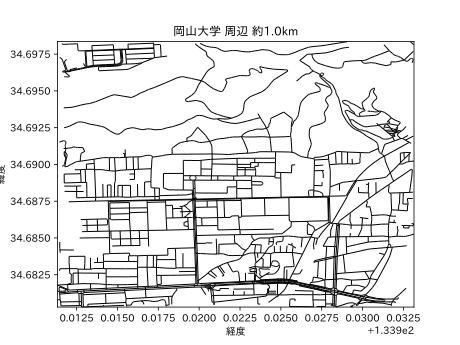
\includegraphics[width=.9\textwidth]{road-ou1.pdf}
  \caption{実験で用いるネットワーク}
  \label{fig:net-ou1}
\end{figure}

ネットワークにランダムな辺を挿入または削除したときの実験結果を表\ref{tab:res-ou1}に示す.$100$回の更新の平均を求めた.結果より,実データに対しては提案手法の方が時間がかかることが分かる.実験に用いたネットワークが,人口ネットワークと比べて密度が小さく,疎なネットワークであることが原因と考えられる.

\begin{table}[tb]
  \centering
  \caption{実データに対する実験結果}
  \label{tab:res-ou1}
  \begin{tabular}{lrr}
    \hline\hline
    更新タイプ & 挿入 & 削除 \\ \hline\hline
    再計算[s] & 0.370 & 0.379 \\ \hline
    更新[s] & 0.748 & 34.576 \\ \hline\hline
    再計算した頂点の割合 & 0.995 & 1.000 \\ \hline\hline
  \end{tabular}
\end{table}
